\section{Applications: Judging Wine Quality}

As a sort of fun application, I found a dataset on UCI's archive from a paper by
Cortez et al. \cite{2009CCAMR} which charted various physicochemical properties
of a set of white wine, and had corresponding 'quality' (judged by a committee,
the CVRVV) levels for each data point. The reason why I decided to try this
dataset, is not only because knowing what makes alcohol quality clearly
a very important task, but also because in the original paper, their uncertainty
regarding the relevancy of all input variables was noted. That is, this is an
interesting opportunity to try a feature selection method: my method of choice
this time was ridge-regression, the $\ell^2$ variant of LASSO. See figures
\ref{fig:linearwine} and \ref{fig:ridgewine} for the linear and ridge regression
variants, respectively.
\begin{figure}[!htb]
  \centering
  \begin{subfigure}{.5\textwidth}
    \centering
    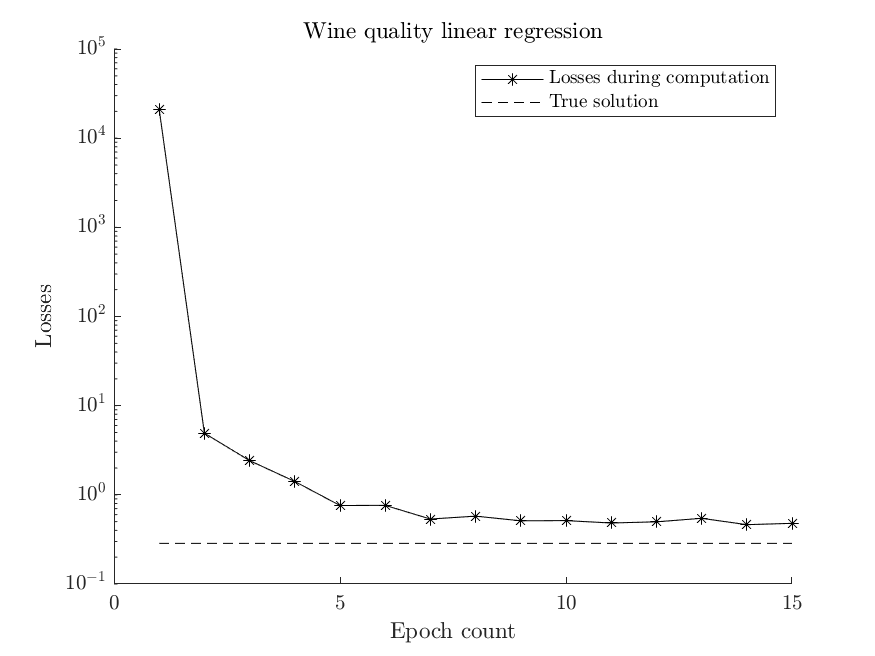
\includegraphics[width=\linewidth]{./resources/linear_wine}
    \caption{}\label{fig:linearwine}
  \end{subfigure}%
  \begin{subfigure}{.5\textwidth}
    \centering
    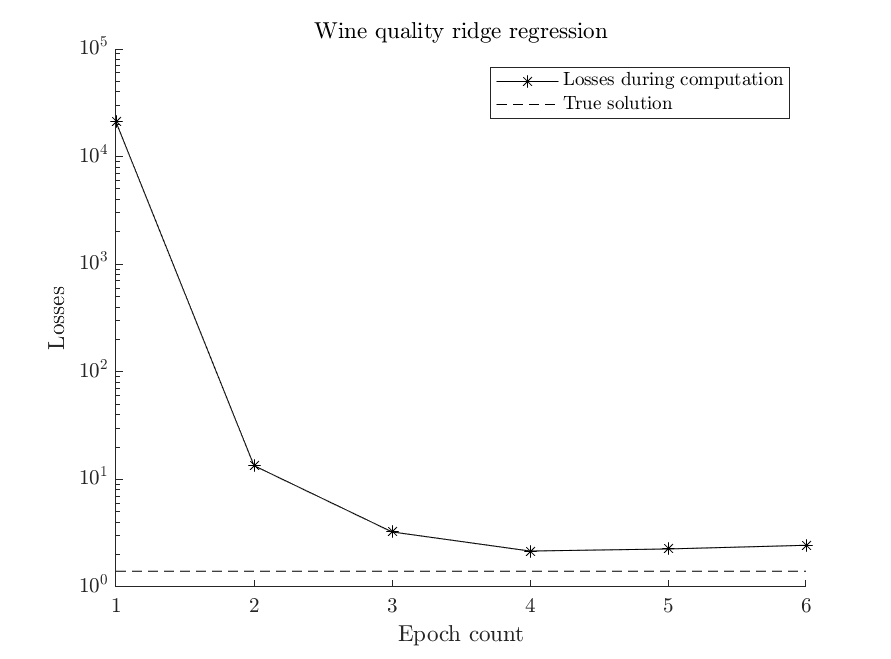
\includegraphics[width=\linewidth]{./resources/ridge_wine}
    \caption{}\label{fig:ridgewine}
  \end{subfigure}
  \caption{
    Both converge in rougly four to eight epochs, but it should be noted
    that neither converges to the true solution. Regardless of how I chose the
    learning rate, it appeared that both runs of \hogwild\ would get stuck in
    a noise ball somewhere close to the true solution. This is an important
    failing of stochastic gradient methods in general, sometimes the noise
    generated will prevent us from seeing a 'true' solution, and indeed the
    ridge-regressed version didn't properly feature select, whereas the solution
    computed via CVX saw the 11th feature to be most weighted (The 11th feature,
    to my amusement, is alcohol content. Certainly an important part of what
    makes a good wine...).
  }
\end{figure}
